% This is "sig-alternate.tex" V2.0 May 2012
% This file should be compiled with V2.5 of "sig-alternate.cls" May 2012
%
% This example file demonstrates the use of the 'sig-alternate.cls'
% V2.5 LaTeX2e document class file. It is for those submitting
% articles to ACM Conference Proceedings WHO DO NOT WISH TO
% STRICTLY ADHERE TO THE SIGS (PUBS-BOARD-ENDORSED) STYLE.
% The 'sig-alternate.cls' file will produce a similar-looking,
% albeit, 'tighter' paper resulting in, invariably, fewer pages.
%
% ----------------------------------------------------------------------------------------------------------------
% This .tex file (and associated .cls V2.5) produces:
%       1) The Permission Statement
%       2) The Conference (location) Info information
%       3) The Copyright Line with ACM data
%       4) NO page numbers
%
% as against the acm_proc_article-sp.cls file which
% DOES NOT produce 1) thru' 3) above.
%
% Using 'sig-alternate.cls' you have control, however, from within
% the source .tex file, over both the CopyrightYear
% (defaulted to 200X) and the ACM Copyright Data
% (defaulted to X-XXXXX-XX-X/XX/XX).
% e.g.
% \CopyrightYear{2007} will cause 2007 to appear in the copyright line.
% \crdata{0-12345-67-8/90/12} will cause 0-12345-67-8/90/12 to appear in the copyright line.
%
% ---------------------------------------------------------------------------------------------------------------
% This .tex source is an example which *does* use
% the .bib file (from which the .bbl file % is produced).
% REMEMBER HOWEVER: After having produced the .bbl file,
% and prior to final submission, you *NEED* to 'insert'
% your .bbl file into your source .tex file so as to provide
% ONE 'self-contained' source file.
%
% ================= IF YOU HAVE QUESTIONS =======================
% Questions regarding the SIGS styles, SIGS policies and
% procedures, Conferences etc. should be sent to
% Adrienne Griscti (griscti@acm.org)
%
% Technical questions _only_ to
% Gerald Murray (murray@hq.acm.org)
% ===============================================================
%
% For tracking purposes - this is V2.0 - May 2012

\documentclass{sig-alternate}
\usepackage{color}
\usepackage[usenames,dvipsnames]{xcolor}
\usepackage{url}

\newcommand{\TODO}[1]{{\color{red} TODO: #1}}
\newcommand{\gametitle}{{\color{RoyalPurple} Dragon Architect Academy}}

\begin{document}
%
% --- Author Metadata here ---
\conferenceinfo{Foundations of Digital Games (FDG)}{2015}
% \pdfinfo{
% /Title ()
% /Author (Aaron Bauer, Eric Butler, Zoran Popovic) 
% /Subject ()
% /Keywords ()
% }
%\CopyrightYear{2007} % Allows default copyright year (20XX) to be over-ridden - IF NEED BE.
%\crdata{0-12345-67-8/90/01}  % Allows default copyright data (0-89791-88-6/97/05) to be over-ridden - IF NEED BE.
% --- End of Author Metadata ---

\title{Visual Programming and Cube-Coding Gooooodtimes}

\numberofauthors{1}
\author{Anonymized}

% \numberofauthors{1} 
% \author{
% \alignauthor
% Aaron Bauer, Eric Butler, Zoran Popovi\'c\\
%        \affaddr{Center for Game Science}\\
%        \affaddr{Computer Science \& Engineering}\\
%        \affaddr{University of Washington}\\
%        \affaddr{Seattle, WA 98195}
%        \email{\{awb, edbutler\}@cs.washington.edu}
% }

\maketitle
\begin{abstract}
\TODO{classy abstract}
\end{abstract}

% A category with the (minimum) three required fields
\category{K.3.2}{Computers and Education}{Computer and Information Science Education -- Computer science education}

\terms{Design, Human Factors}

\keywords{Game-based learning; computational thinking; programming education}

\section{Introduction}
The past few years have seen many efforts to broaden the reach of computer science education and make it available, and appealing, to more students in more places. 
Many of these projects, including some of the most visible such as Scratch and Code.org's Hour of Code~\cite{codedotorg}, are online programming environments that expose users to basic programming concepts. 
Despite the proliferation of these systems, little work has investigated the design of the structure or content of such systems. 
Comparative studies providing evidence for effective ways of presenting these ideas in this context have been largely absent. 

A Potential line of inquiry could include the effects of changes in programming language syntax and semantics on novices. 
One might ask if there are benefits to evolving the available language elements as a novice progresses, and in which order these elements should become available. 
What combination of language elements affords beginners the most expressiveness without introducing overwhelming complexity? Another set of questions concern the impact of combining puzzles and an open-ended sandbox. 
Can puzzles provide sufficient structure and guidance to facilitate productive exploration of a game's concepts in an unstructured sandbox? 
When and how should the player transition between the two? 
These and many more topics relating to online programming environments deserve further study, particularly in light of their surging popularity \TODO{footnote about \# of Scratch users/Hour of Code participants?}. 

In this paper we present \gametitle{}, an educational game designed to be a tool with which to conduct such studies. 
In \gametitle{}, players use a visual, drag-and-drop programming language to control a dragon in a 3D grid world. 
The visual language is a set of \emph{code blocks} that snap together to form programs. 
The player can move the dragon in three dimensions and have the dragon place and remove cubes of various colors. 
In addition to blocks that control the dragon directly, players can also make use of definite loops and procedures (see Figure~\ref{fig:toolbox}).

\begin{figure}[ht]
  \centering
  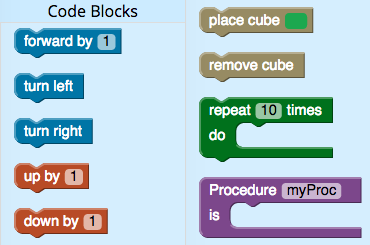
\includegraphics[width=\columnwidth]{images/toolbox_wide}
  \caption{The programming elements currently available in \gametitle{}}
  \label{fig:toolbox}
\end{figure}

Our motivation for developing \gametitle{} is to use it in exploring a variety of open questions in both education and games. 
The remainder of this paper is as follows: after \gametitle{} is described in more detail, it surveys the related work and discusses the related learning theory. 
Next, it discusses our research goals. 
The paper then highlights several design issues that have arisen during \gametitle{}'s development and presents our observations from students' experiences with the game so far. 
The paper concludes with our thoughts on other interesting questions our system might be used to answer.

\section{\gametitle{}}
\TODO{Can't use macros in section titles because the formatted gets messed up, replace once we choose a title}
We have been developing \gametitle{} since spring 2014. 
\gametitle{} is played in a web browser, and similar to many other such systems, the page is separated into two parts: an area where the player can assemble their code and a visualization of the environment their code affects (\TODO{figure}). 
The visualization uses the Unity game engine~\TODO{cite} and the drag-and-drop programming UI is provided by the Blockly library~\TODO{cite}.

\subsubsection{Progression}

As they progress through the game, players alternate between short sequences of one to five puzzles with a specific goal and a specific set of available code blocks and an open-ended sandbox. 
The game begins with four puzzles that introduce the idea of assembling and running code, as well as the code blocks for moving the dragon in 2D and putting down cubes.
After that, the player can experiment and build in the sandbox and complete other puzzle sequences to make more code blocks available in the sandbox, switching between sandbox and puzzles at any time. 
Like the first puzzles, each subsequent sequence focuses on a few specific concepts. 
In this way, the language the player uses to write instructions for the dragon gradually expands as the player advances.

% \subsubsection{Language}

% The visual, drag-and-drop language used by the player is a custom, if, in game's development so far, simplistic, language designed specifically for \gametitle{}. We have implemented a textual concrete syntax, and we plan for the game to eventually expose this to the player, allowing them to choose which input method they prefer. This also allows for a direct translation from text to code blocks and vice versa. Some similar projects use a popular industry programming language such as Javascript or Java. We believe implementing our own gives us a valuable flexibility as well as preventing our players from dealing with the idiosyncrasies of any popular language. Having complete control over every part of the language implementation will provide useful in any study of the effects of changes in language features. 

% \subsubsection{Technology}
% \TODO{a few sentences or cut}


\section{Related Work}
The tremendous and recent proliferation, in both quantity and variety, of online programming environments attempting to teach or promote engagement with computer science ideas, especially basic programming concepts, has greatly informed the development of \gametitle{}. In some, like the step-by-step lessons available from Khan Academy~\cite{khanacademy} and Codecademy~\cite{codecademy}, or the game CodeSpells \cite{esper2013codespells}, users program in a popular industry programming language such as Javascript or Java. Given that syntax can be an obstacle for those new to programming~\cite{stefik2013syntax}, however, we chose to use a visual language as there is evidence those are helpful to novices~\cite{whitley1997visual}. \TODO{should also mention Programming By Design and related project Bootstrap as curricula-oriented projects}

Of any one source, \gametitle{} takes the most inspiration from Scratch~\cite{maloney2010scratch}, a visual programming environment focused on empowering its users to create interactive digital media.
\begin{itemize}
\item Scratch~\cite{maloney2010scratch} -- basis for drag-and-drop language; successful in building vibrant community around open-ended, creative, social environment (want to borrow ideas of personalization in the future); lack of structure may pose a barrier to entry and to learning (quantity and complexity of immediately available features may be intimidating or confusing, discovery-learning-ineffective citation); with \gametitle{} we want to see if a gradual introduction of features can be easier to get in to while still inspiring the creative experimentation Scratch fostered in its community
\item Code.org -- Hour of Code very visible, but limited in scope and expressiveness (linear sequence of puzzles); our goal is to provide a much longer engaging experience where players can explore both broadly and deeply
\item \cite{zorn2013minecraft} -- building upon Minecraft's capacity for broad engagement
\end{itemize}

\TODO{disconnected related work sentences}

Kelleher and Pausch review programming environments for novices and describe a taxonomy of these systems~\cite{kelleher2005lowering}. Within that taxonomy, \gametitle{} fist best as a teaching system that targets \emph{structuring programs} and aims to provide learning support both through \emph{social learning} and \emph{providing a motivating context}.

Lye and Koh recently reviewed studies investigating teaching computational thinking in K12 classrooms~\cite{lye2014review}. They found that this area deserves more research. In particular, the reviewed findings suggest structured, guided discovery is a better approach for learning than pure self-driven discovery.

\emph{BOTS} is a programming puzzle game. The stated goal of the project is to study how community-athored content is used in educational games~\cite{hickspart14}, and it has also been used to explore hint generation~\TODO{cite}.


\section{Research Goals}
\label{sec:goals}
Our primary goal for \gametitle{} is to produce a flexible system that we can use to investigate questions in computer science education and game-based learning. These could include studying how to facilitate the transition from a visual programming language to a textual one or the use of puzzles as direct guidance in an educational system. We are especially concerned with these questions as they relate to novice programmers, so we have tried to make \gametitle{} accessible to players as young as 9.

To serve its purpose as a research tool, \gametitle{} needs to be able to attract and engage a population of players. Getting the project to this point is where the bulk of our development efforts have been focused to date. It may have been possible to avoid this investment in large part by using an existing piece of educational software. For the kinds of questions we hope to address, however, a high degree of control over both the UI and the language used in \gametitle{} is very beneficial, and is afforded only by developing the system ourselves. While many online programming environments try to teach some of the same ideas our game tries to teach, we know of no other system being used to study the questions we wish to study. 

\subsection{Scaffolded Sandbox}
Within the context of investigating game-based learning, we specifically want to explore the coupling of highly structured puzzle levels and an open, unstructured sandbox. The former unlock and introduce concepts and tools that are then available in the latter. \TODO{citations about creativity being engaging, and pure discovery learning being lousy}. Thus, we aim to use \gametitle{} to study the properties of introducing both structure and direct guidance into a sandbox environment through puzzles. Related questions include to what degree the player should have control over the rate and sequence of puzzles, and effects of introducing social features into this structure. 

\subsection{Directly Teach Strategies}

Beyond basic programming concepts, many have advocated for the greater presence of computational thinking~\cite{wing2008computational} in computer science education (and education in general). It is our goal with \gametitle{} to approach teaching these ideas in a more profound way then simply hoping students absorb this \emph{way of thinking} as a byproduct of working with other computer science concepts (such as basic programming). We propose to go further and teach computational thinking by directly teaching one of its core components: the identification and application of problem-solving strategies (such as divide and conquer). 

A great deal of recent education research suggests that \emph{curricula can model such strategies for students} and that appropriate guidance, which in many cases consists of the capabilities afforded by a suitable computational environment, can \emph{enable students to learn to use these strategies independently}~\cite{report2010computational}. Mayer and Wittrock~\cite{mayer1996handbook} call attention to the substantial evidence in the education literature for teaching what they call \emph{domain-specific thinking skills} and \emph{metacognitive skills}. The former would include the ability to use a strategy like divide and conquer, and the latter would include knowing when and where to employ that strategy. In both cases, studies have shown that teaching these skills directly can improve learning and performance. 

Our goal is to incorporate computational thinking strategies into the content of an educational game. This includes demonstrating these strategies and giving players an opportunity to practice them. We believe a game is particularly well suited to this task. \TODO{expand on this}


\section{Design Issues}


\subsection{Permanence vs. Experimentation}

\subsection{Flexible Puzzles}


\section{\gametitle{} in Action}
\begin{itemize}
\item how we have made our observations
\item what we have observed
\begin{itemize}
\item kids excited by premise
\item some want to do puzzles, some want to play in the sandbox
\item idea generation (i.e. what to do) in the sandbox can be a barrier
\end{itemize}

\item what we have learned from watching \gametitle{} in action
\end{itemize}


\section{Discussion}
\TODO{description of open problems in CS education and game-based learning, exploration of how \gametitle{} might be used to approach them}

% Comment out in submission version
%\section{Acknowledgments}
%\TODO{copy from CHI papers?}

\bibliographystyle{abbrv}
\bibliography{ruthefjord-fdg-2015} 
\end{document}